Now we have to build our .NET Core Web Application to the specified folder, say \texttt{/mango-linux-build/src}.
Note that it is much better to build it on behalf of Windows 10 main machine, not WSL 2.0 one.
We use the following commands to build .NET Core Web App with \texttt{Release} configuration
\begin{itemize}
    \item \texttt{cd E:/RiderProjects/MangoMessengerAPI/MangoAPI.Presentation}
    \item \texttt{dotnet publish "MangoAPI.Presentation.csproj" -r linux-x64 \\ -o /mango-linux-build/src}
\end{itemize}
Terminal output is as follows
\begin{figure}[H]
    \centering
    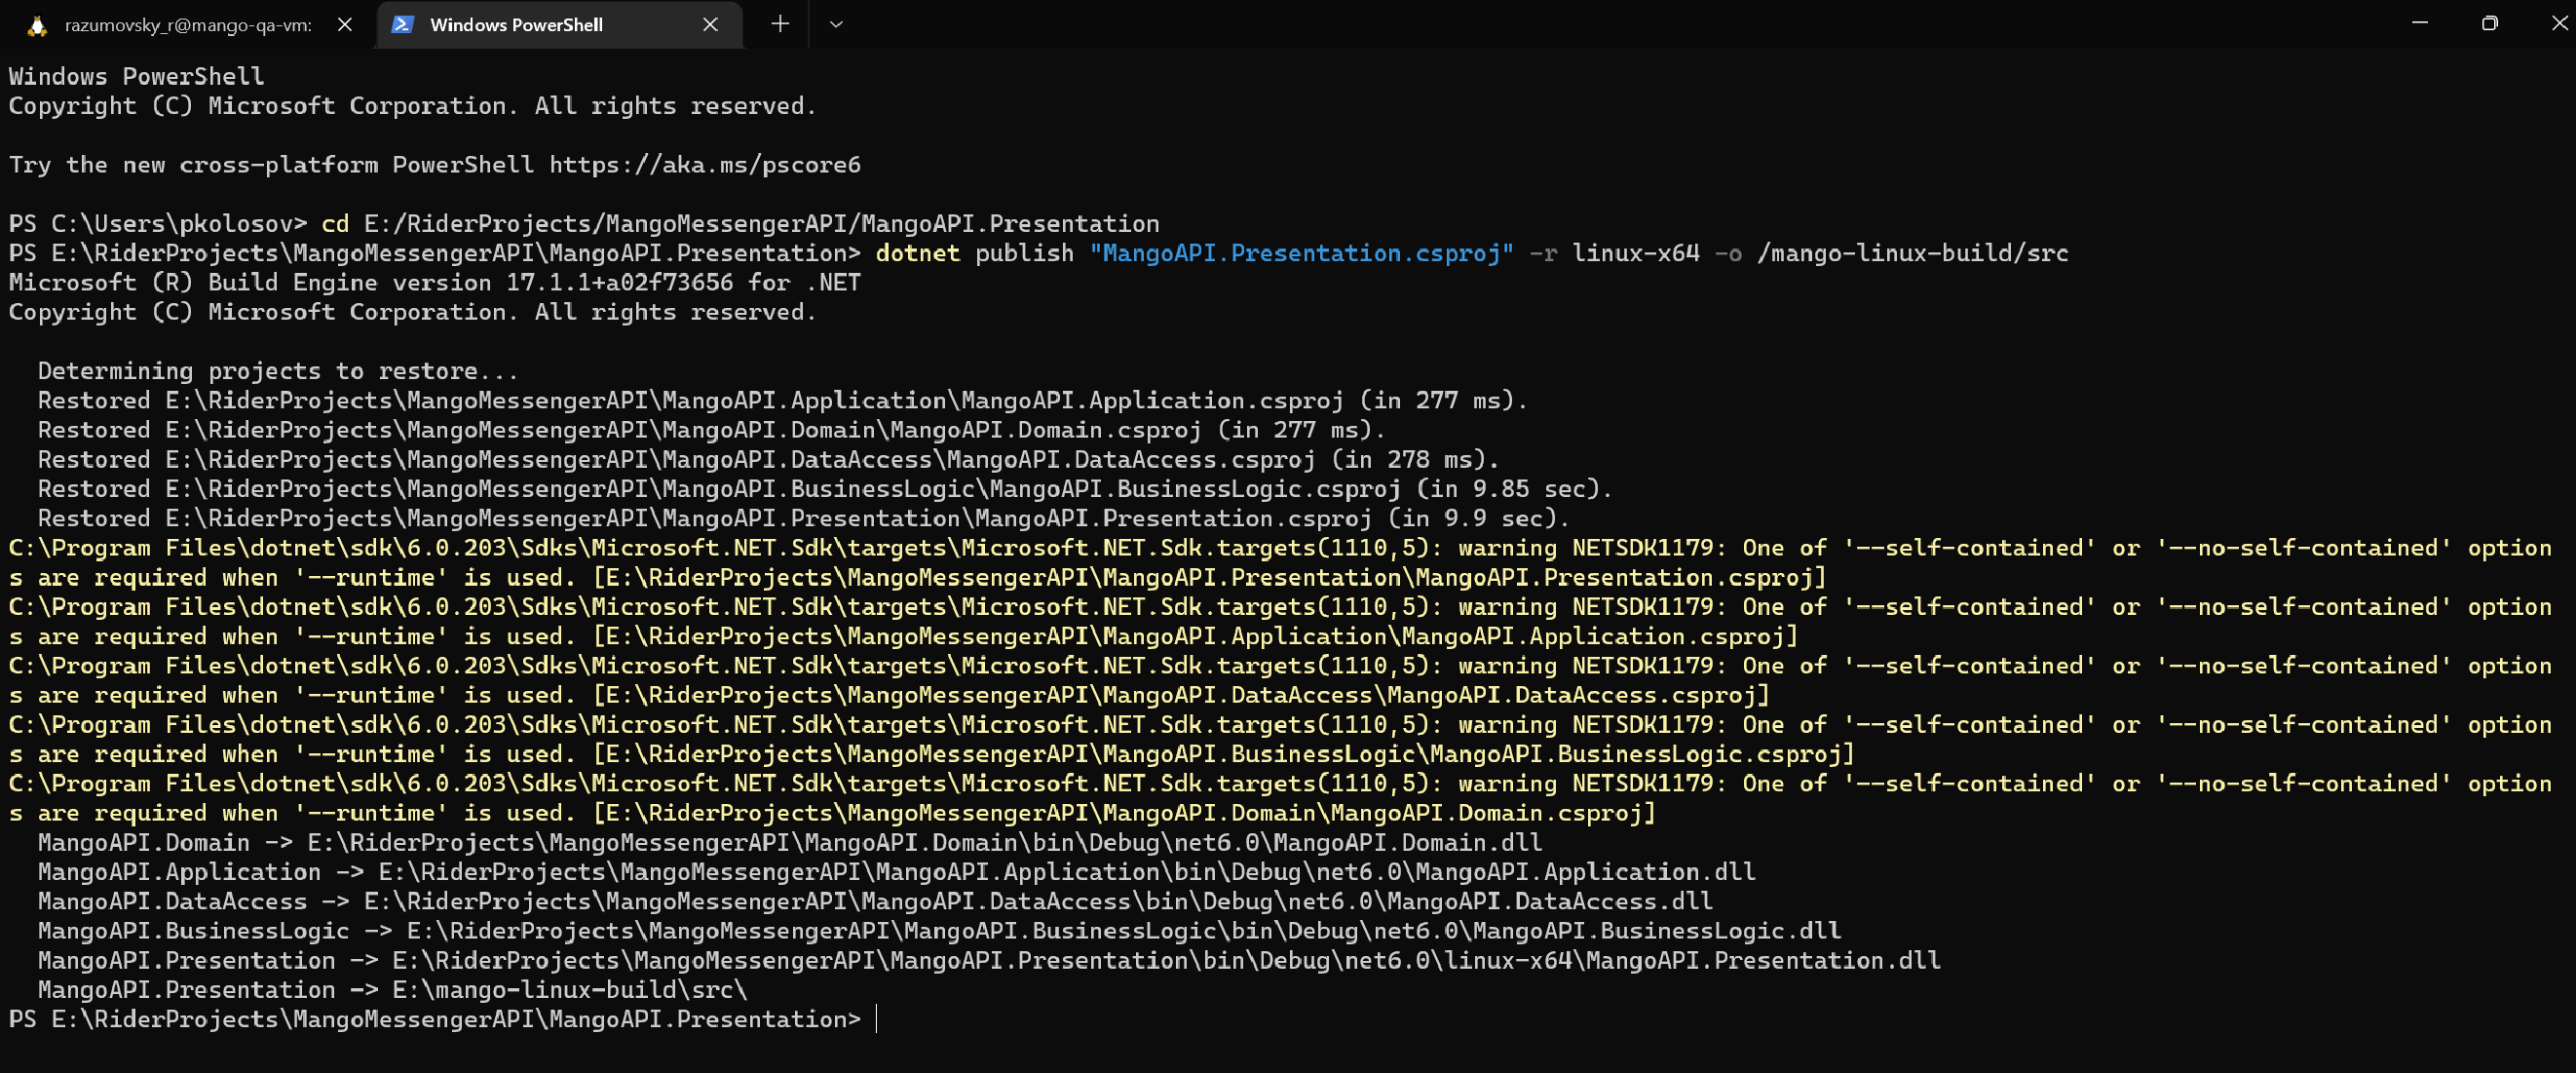
\includegraphics[width=1\textwidth]{img/04_build_application}
    ~\caption{Publish .NET Web app terminal output.}\label{fig:figure9}
\end{figure}
Let's create the folder \texttt{mango-backend} where build files to be stored.
Do not forget to connect to your Azure VM via SSH\@.
Do not also forget to assign read-write privileges to the folder, using the commands
\begin{itemize}
    \item \texttt{sudo mkdir ~/mango-backend}
    \item \texttt{sudo chmod a+rwx ~/mango-backend}
\end{itemize}
Terminal output:
\begin{figure}[H]
    \centering
    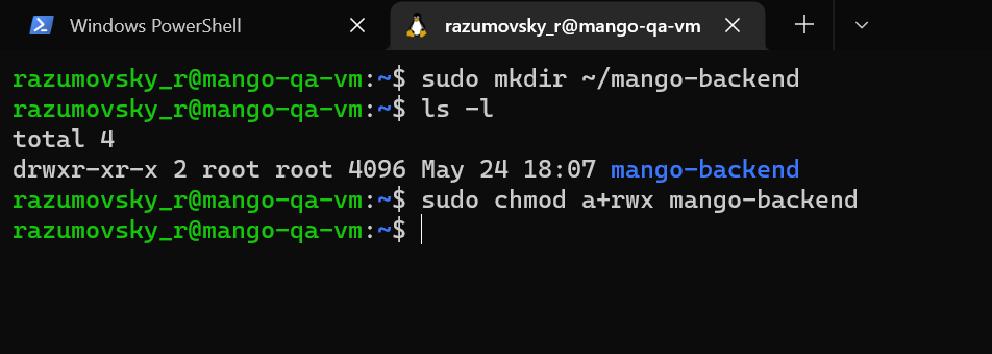
\includegraphics[width=1\textwidth]{img/04_create_remote_folder}
    ~\caption{Create folder at remote VM.}\label{fig:figure10}
\end{figure}
As next step consider to copy build files to the remote folder on your Azure VM so that we execute our program after.
We copy the build files on behalf of WSL2 this time.
In order to copy the build files we use following commands
\begin{itemize}
    \item \texttt{cd /mnt/e/mango-linux-build}
    \item \texttt{scp -r -i ~/.ssh/id\_rsa ./src/* \\ razumovsky\_r@VM\_IP\_ADDRESS:/home/razumovsky\_r/mango-backend}
\end{itemize}
where \texttt{id\_rsa} is the private key.
Terminal output:
\begin{figure}[H]
    \centering
    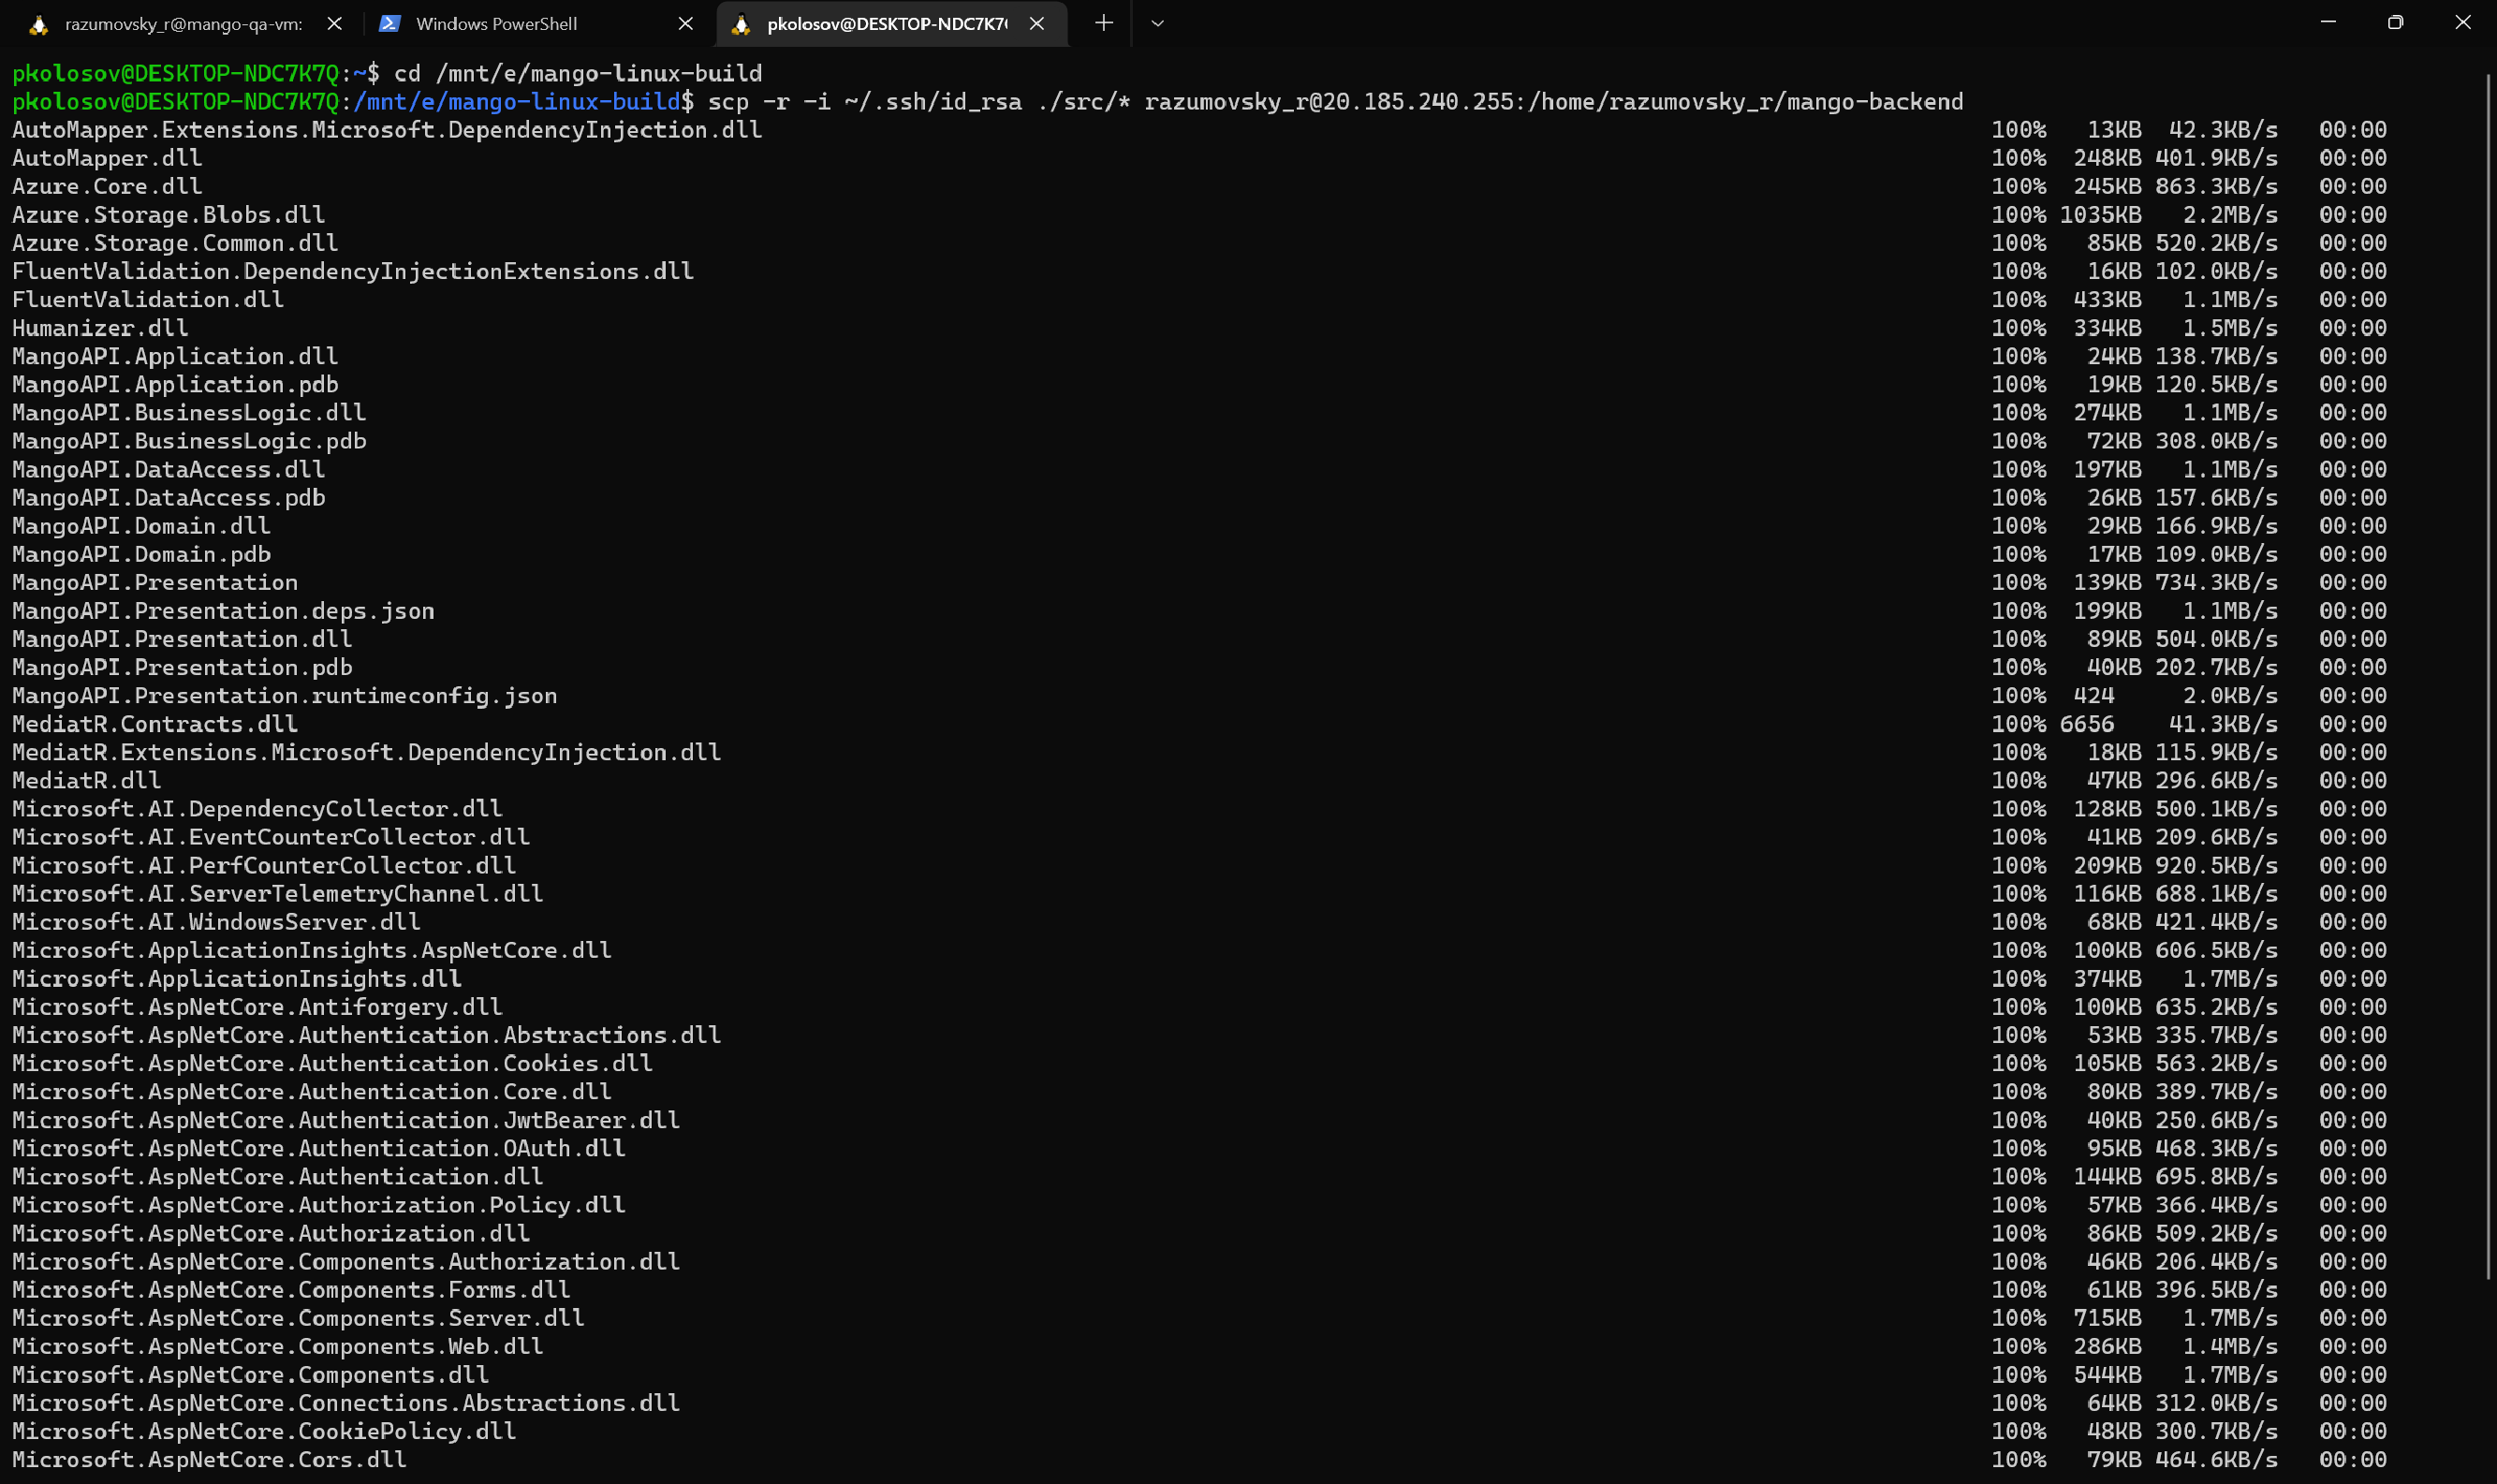
\includegraphics[width=1\textwidth]{img/04_copy_build_files_via_ssh}
    ~\caption{Copy build files via SSH.}\label{fig:figure11}
\end{figure}
Ensure build files are copied successfully to the remote VM, use the command \texttt{ls -l mango-backend}.
Terminal output:
\begin{figure}[H]
    \centering
    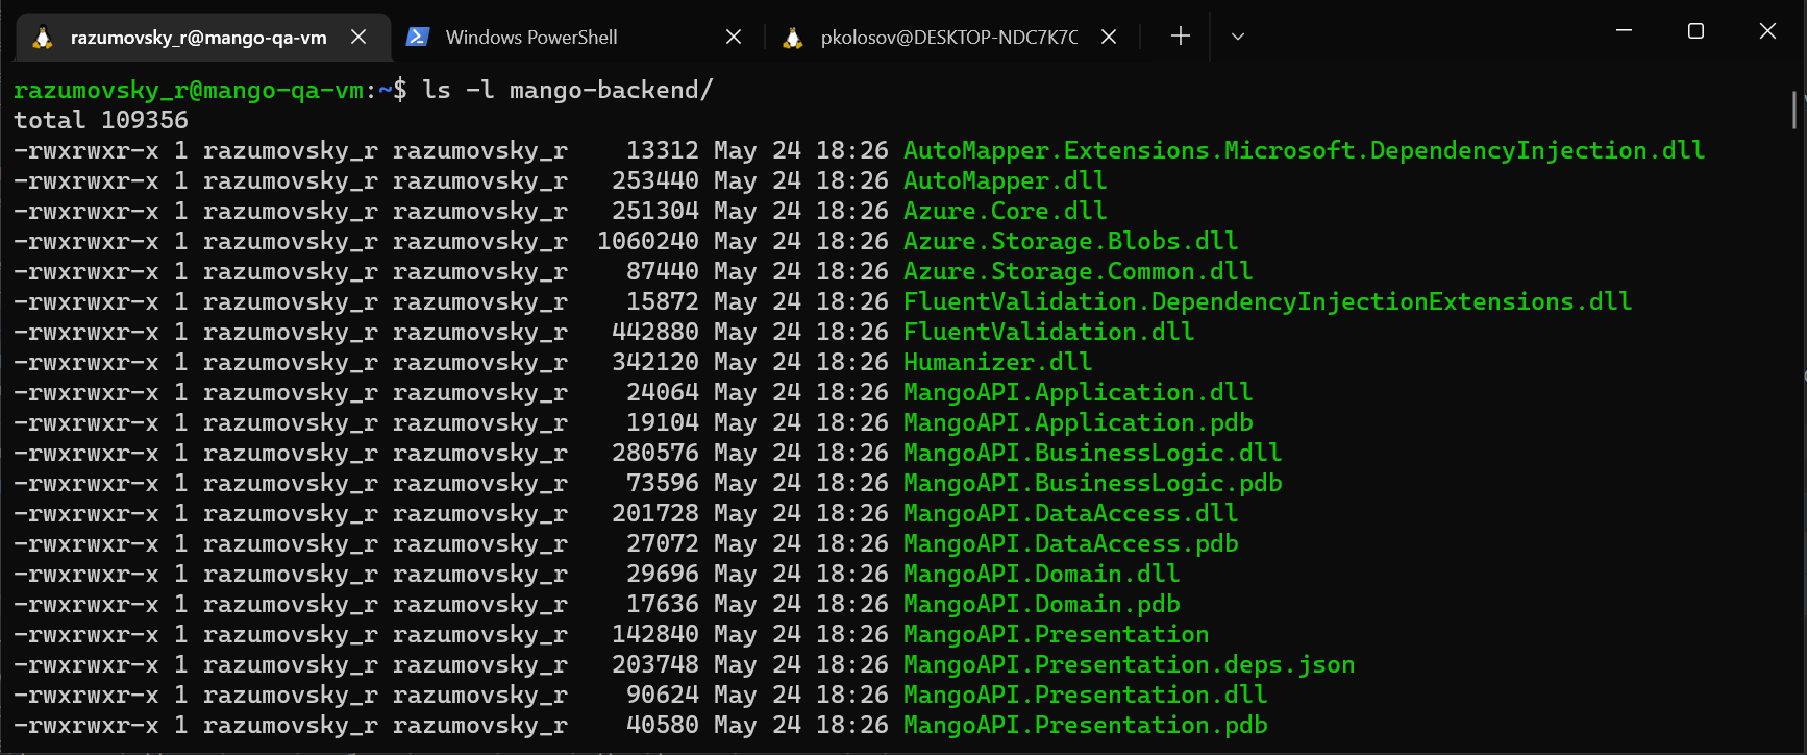
\includegraphics[width=1\textwidth]{img/04_verify_files_on_remote_vm}
    ~\caption{Check files at remote VM.}\label{fig:figure12}
\end{figure}

